\documentclass[11pt]{article}
\usepackage[a4paper, total={6in, 9.5in}]{geometry}
\usepackage[natbibapa]{apacite}
\usepackage[english]{babel}
\usepackage[utf8]{inputenc}
\usepackage{pythonhighlight}
\usepackage{subcaption}
\usepackage{hyperref}
\usepackage{setspace}
\usepackage{setspace}
\usepackage{palatino}
\usepackage{graphicx}
\usepackage{multirow}
\usepackage{titling}
\usepackage{amsmath}
\usepackage{amssymb}
\usepackage{lscape}
\usepackage{float}

\fontfamily{ppl}\selectfont 
\renewcommand{\baselinestretch}{1.5} 
\bibliographystyle{apacite}
\onehalfspacing
\setlength{\droptitle}{-5em}

\title{Prevent overcrowding in exhibitions using FogFlow to distribute people}

\author{Lorenzo Siega\\
    \href{mailto:lorenzo.siega@mail.polimi.it}{\texttt{lorenzo.siega@mail.polimi.it}}
}

\date{\today}

\begin{document} {
    \setstretch{.8}
    \maketitle
    
    \begin{abstract}
    The organizers of an exhibition with several booths are trying to avoid overcrowded booths so visitors could be distributed smoothly and enjoy the exhibition. They mount cameras at each booth so to know the number of people currently at each booth.\\
    Each booth has an electrical board which, based on the information from other booths their distance, suggests visitors the closest booth to visit next in a way that the population is smoothly distributed.\\
    The overall number of visitors of each booth is reported to the cloud for information aggregation to be queried for the crowded time of the day.
    \end{abstract}
}

\section{Introduction}
During an exhibition with several booths people can stop in front of a booth and create a congestion. By providing them informations about the next more suitable booth to visit, we can distribute them more efficiently.\\
People at each booth are counted using cameras and then an algorithm suggest, for each both, a booth to visit by displaying it on an electrical board.
To archive that we have to face two main problems:
\begin{itemize}
    \item Required analysis effort: As we have to analyze a stream of images from an unknown number of cameras, we can't compute on a centralized component.
    \item Algorithm: Algorithm works on the entire set of booths and triggering it on each update received from a booth, as FaaS computing does, will generate an high computation and data load.
\end{itemize}{}
FogFlow can address to both problems, by filling these gaps:\\
\begin{quote}
    \begin{enumerate}
        \item[G2] Function triggering: from per event to per selected entities: In existing serverless computing frameworks, functions are invoked per event with limited execution time and memory size. This is not suitable for data-intensive IoT services.[...]
        \item[G3] Function execution: from data $\rightarrow$ code or code $\rightarrow$ data to code $\leftrightarrow$ data: Existing serverless computing frameworks separate data management from the function execution environment, always moving data into the execution environment for function execution (data to code pattern). On the other hand, existing fog computing frameworks such as Azure IoT Edge move cloud functions to the data located at the edges.[...]
        \item[G4] Function composition: from event-oriented or edge-oriented to data-centric: 
        In existing serverless computing frameworks such as OpenWhisk, service developers need to customize a series of event triggers and rules to link multiple functions together. Existing fog computing frameworks allow service developers to link functions at each edge by manually configuring the topic-based data routing path between them.[...]
    \end{enumerate}{}
\end{quote}
\cite{cheng2019fog}
\begin{figure}[h]
    \centering
    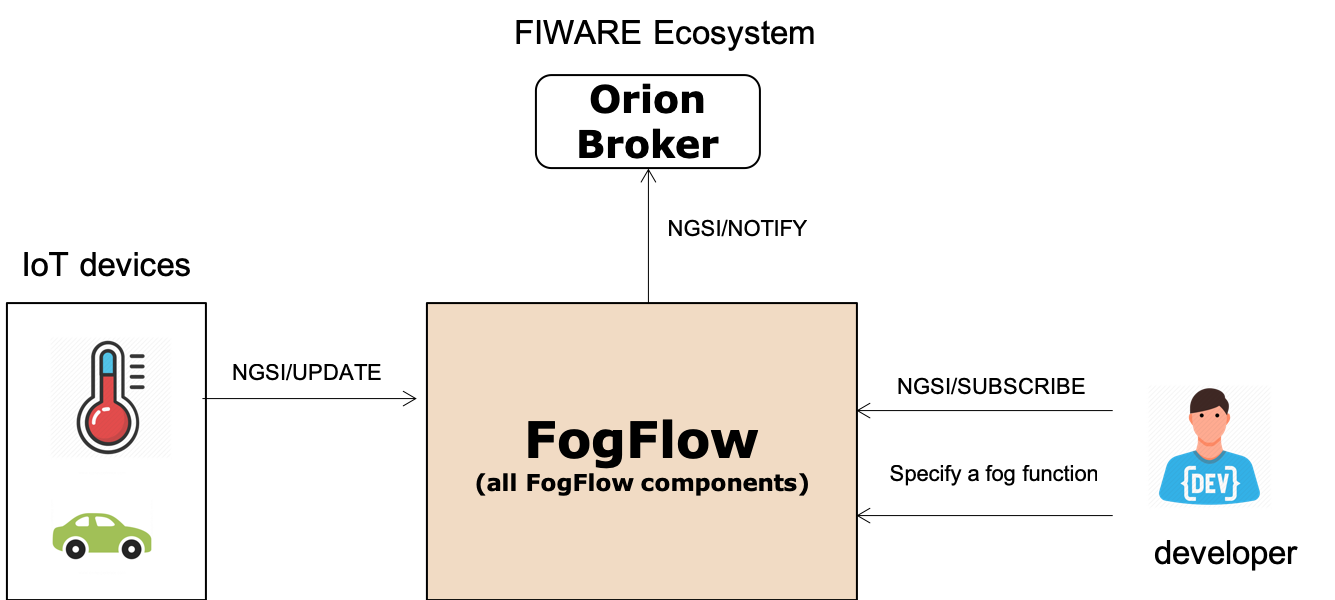
\includegraphics[width=0.7\textwidth]{Images/systemview.png}
    \caption{System view}
\end{figure}{}

\section{Context producers vs. context consumers}
At each booth will be deployed:
rapberry pi as broker/context-producer/context-comsumer
one or more cameras.

\begin{python}
import openface

align = openface.AlignDlib('/root/openface/models/dlib/shape_predictor_68_face_landmarks.dat')

def faceCounting(url):     
    image = url2Image(url)
    if image is None:
        raise Exception("Unable to load image: {}".format(url))
        
    faces = align.getAllFaceBoundingBoxes(image)
    if faces is None:
        raise Exception("Unable to find a face: {}".format(url))

    now = datetime.datetime.now().strftime("%Y-%m-%d %H:%M:%S")      
    result = {"date": now, "facenum": len(faces), "totalbytes": total_size}    

    return result
    
def publishResult((result):
    resultCtxObj = {}
        
    #annotate the context with the configured entity id and type
    if len(outputs) < 1:
        return   
    
    resultCtxObj['entityId'] = {}
    resultCtxObj['entityId']['id'] = outputs[0]['id']
    resultCtxObj['entityId']['type'] = outputs[0]['type']        
    resultCtxObj['entityId']['isPattern'] = False    
    
    resultCtxObj['attributes'] = {}
    resultCtxObj['attributes']['num'] = {'type': 'integer', 'value': result['facenum']}
    resultCtxObj['attributes']['totalbytes'] = {'type': 'integer', 'value': result['totalbytes']}    

    # publish the real time results as context updates    
    updateContext(resultCtxObj)
    
publishResult(faceCounting(image))
\end{python}

\begin{figure}[h]
    \centering
    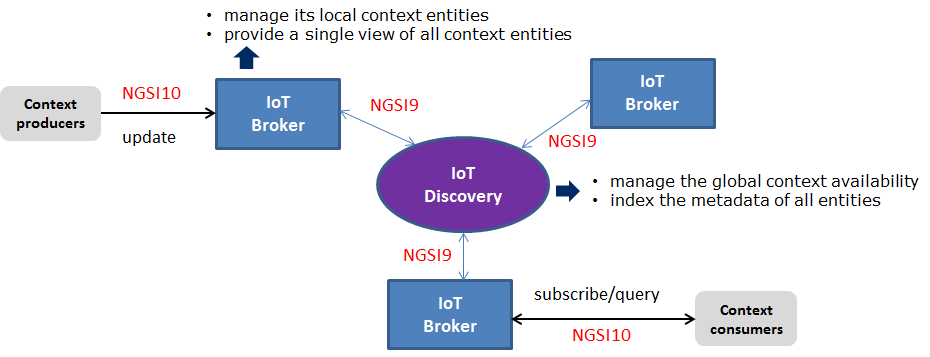
\includegraphics[width=0.9\textwidth]{Images/distributed-brokers.png}
    \caption{System view}
\end{figure}{}

\section{Operator}
Operator code must be in the form of a docker image and must be available on docker hub.

FogFlow enables serverless edge computing, meaning that developers can define and submit a so-called fog function and then the rest will be done by FogFlow automatically, including:

triggering the submitted fog function when its input data are available
deciding how many instances to be created according to its defined granularity
deciding where to deploy the created instances

The instances in the above text refer to the task instances which run a processing logic within them and this processing logic is given by operators in fogflow. They must be registered beforehand by the users. Implementation of an example operator is given in the next sections.

\section{Topology}
In FogFlow a service topology is defined as a graph of several operators. Each operator in the service topology is annotated with its inputs and outputs, which indicate their dependency to the other tasks in the same topology. Different from fog functions, a service topology is triggered on demand by a customized “intent” object.

Once developers submit a specified service topology and the implemented operators, the service data processing logic can be triggered by following two steps:

Sending a high level intent object which breaks the service topology into separate tasks
Providing Input Streams to the tasks of that service topology.
The intent object is sent using the fogflow dashboard with the following properties:

Topology: specifies which topology the intent object is meant for.
Priority: defines the priority level of all tasks in your topology, which will be utilized by edge nodes to decide how resources should be assigned to the tasks.
Resource Usage: defines how a topology can use resources on edge nodes. Sharing in an exclusive way means the topology will not share the resources with any task from other topologies. The other way is inclusive one.
Objective: of maximum throughput, minimum latency and minimum cost can be set for task assignment at workers. However, this feature is not fully supported yet, so it can be set as “None” for now.
Geoscope: is a defined geographical area where input streams should be selected. Global as well as custom geoscopes can be set.

\begin{figure}[h]
    \centering
    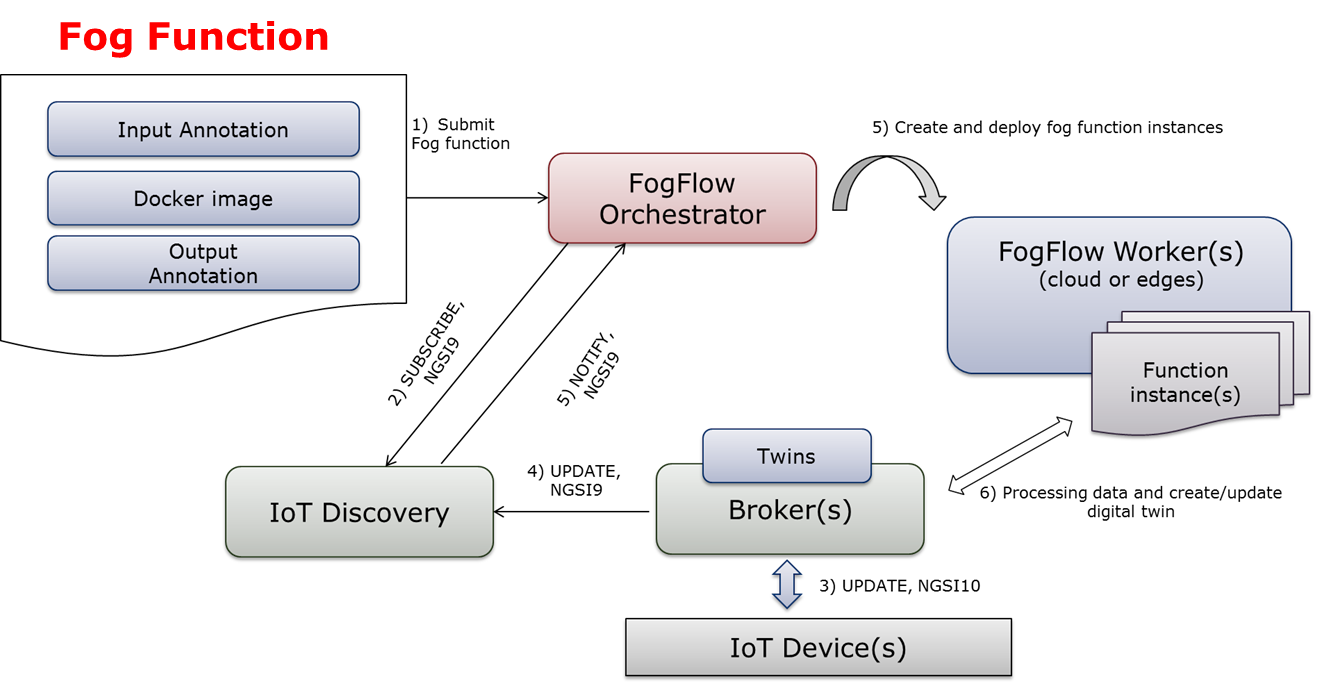
\includegraphics[width=0.7\textwidth]{Images/function-orchestration.png}
    \caption{System view}
\end{figure}{}
\section{Distribution fog function design}
\section{Testing}

\bibliography{main}
\end{document}